\section{Results}
In this section we first briefly discuss the general flow of our implementation. Then we will explain the used methods and results for each question from before. We based our solutions on the findings in the previous literature study \cite{literatuurstudie}. Our solution is implemented in Java using the Weka toolkit \cite{Weka}.

\subsection{General Flow}
The implementation that tries to achieve our goal follows the sequence showed in Figure ~\ref{flow}.
First both the training data and testing data are parsed from their corresponding CSV-files.
Secondly these datasets are split up into different windows. Then a Feature Extractor will extract all useful features from these windows. Next a filter is used to filter out corrupt windows based on these features. Then the training data will train a classifier. This classifier will on its turn classify all the filtered testwindows.
Finally all these windows then need to be recombined to one walk by voting for their classifications. This will in the end generate the result.

\begin{figure}[ht]

\centering
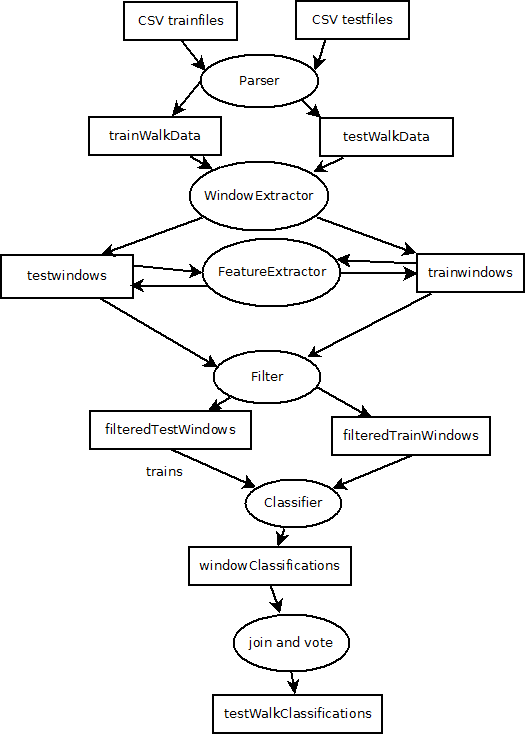
\includegraphics[scale=0.5]{flow.png}
\caption{General work flow of solution}\label{flow}
\end{figure}

\subsection{Windows}
We used sliding windows with 50\% overlap for feature extraction since this has been demonstrated succesfull in past works \cite{bao2004activity}. Our solution uses a sampling frequency of 50 Hz and each window represents 5.1 seconds. This way every window has at least 256 samples. A window of several seconds
was used to sufficiently capture cycles in the walking \cite{bao2004activity}.
We also tried to use windows of 2.55 seconds but this proved to give worse results.

\subsection{Features}
In total we extract 42 features for each window. We use a combination of time and frequency domain features that have given good results in previous papers \cite{bao2004activity}\cite{preece2009comparison}. 
All the features are computed for each axis except for the correlation which is determined by using every combination of two axes.The number in brackets indicates the number of features that are extracted.
\begin{itemize}
  \item Mean (3), standard deviaton (3), median (3), first and third percentile (6)
  \item minimum (3), maximum (3)
  \item Correlation between the axes (3)
  \item Magnitude of first 5 components of FFT analysis (15)
  \item Energy (3)
\end{itemize}

\subsection{Filter}
As mentioned in the assignment it is possible that certain windows will contain corrupt data. (e.g. generated when starting the sensors) Therefore we provide the possibility to create a filter to remove unwanted windows from both test and training set.
This filter is based on a second classifier which aims to classify corrupt windows as unwanted.
When the \textit{manualfilter} command is given to the terminal, a screen will pop up showing a plot for the values of a window. The user can then either accept or reject this window. Then a next window will appear that the user has to manually classify. This process continues as long as the user wants.
Based on the decisions the user made, a Decision Tree classifier will be trained.
This classifier will than behave as a filter for all the remaining windows.

The created filter however did not seem to provide noticable added accuracy for all classifiers. For the nearest neighbor classifier the accuracy did go up. The fact that it did not add accuracy to the other classifiers might however be caused because of the poor quality of the results before adding the filter (See \ref{result}).

\subsection{Assessing Accuracy}
To assess the accuracy of our solutions, we use leave-one-out cross-validation.
(Results can be shown with the \textit{crossvalidation} command). Cross-validation however requires independence between training and test set. This poses a problem if we were to use it directly on the windows because of the overlap. Therefore cross-validation is performed on entire walks.\\
An entire walk is classified by letting each of the classified windows vote for the classification they think is the best one. Each vote is weighted by the corresponding confidence.\\
If the \textit{crossvalidation} command is given the system will print out for each known person as which person he was qualified and how many times. 

\subsection{Classification}
The classifier mentioned in this section is the one used to classify windows as a person.
Our solution has the ability to use every Weka classifier with every allowed option. We did however provide additional functionality for the following classifiers since these were used extensively in related work. In italics are the corresponding Weka classifiers if their name does not correspond
  \item Decision Trees (\textit{J48})
  \item Support Vector Machines (\textit{SMO})
  \item k Nearest Neighbors (\textit{Ibk})
  \item Naive Bayes 
  \item Random Forest
\end{itemize}

\subsection{Overall Result}\label{result}
All the used classifiers classify most, if not all test data as ``Other''.
This is not in se a bad thing, but we do not know why this happens. 
The cross-validation of the set of training walks gives the same result (it predicts a lot of ``Other'' classes).
What follows is an overview of the different classifiers that were used in previous works. For these we provided a shortcut in the commandline. The arguments that are displayed in each subsection are the arguments that were given to our program. According to the accuracy the nearest neighbor classifier performs best with an accuracy of 73.6\%. Therefore it is the default classifier.

\subsubsection{Trees}
Arguments : -d -cm -cv -c tree
\paragraph{Cross validation}
General accuracy of : 62.2\%\\

other classified as : other(29) leander(3) wannes(2) \\
leander classified as : other(6) leander(1) \\
wannes classified as : other(8) leander(1) wannes(3) 

\paragraph{Confusion matrix for windows}

\begin{tabular}{l l l | l}
    a &    b &   c & $\leftarrow$ classified as \\
    \hline
   791 & 5 & 6 &    a = other \\
    3 &  120 &  0 &    b = leander \\
    6 &   2 &  64 &    c = wannes
\end{tabular}

\paragraph{Classification}
\begin{tabular}{l | l | l}
    file & result & confidence\\ 
    \hline 
    walk\_59\_unknown.csv & Wannes   & $0.45098039215686275$ \\
    walk\_60\_unknown.csv & Other   & $0.9905660377358491$ \\
    walk\_61\_unknown.csv & Other   & $0.620507925999485$ \\
    walk\_62\_unknown.csv & Other   & $0.70947389437955476$ \\
    walk\_63\_unknown.csv & Other   & $0.7036363636363636$ \\
    walk\_64\_unknown.csv & Wannes   & $0.8571428571428571$ \\
    walk\_65\_unknown.csv & Wannes  & $0.5257142857142857$ \\
    walk\_66\_unknown.csv & Other   & $0.8731768417931942$ \\
    walk\_67\_unknown.csv & Other  & $0.6641975308641975$ \\
    walk\_68\_unknown.csv & Other   & $0.9224150943396229$
\end{tabular}

\subsubsection{Naive bayes}
Arguments : -d -cm -cv -c nbayes 
\paragraph{Cross validation}
General accuracy of : 28.3\%\\
other classified as : other(1) leander(29) wannes(4) \\
leander classified as : leander(7) \\
wannes classified as : other(1) leander(4) wannes(7) 

\paragraph{Confusion matrix for windows}

\begin{tabular}{l l l | l}
    a &    b &   c & $\leftarrow$ classified as \\
    \hline
   20 &  649 & 133 &    a = other \\
    0 &  118 &   5 &    b = leander \\
    1 &   10 &  61 &    c = wannes
\end{tabular}

\paragraph{Classification}
\begin{tabular}{l | l | l}
    file & result & confidence\\ 
    \hline 
    walk\_59\_unknown.csv & Leander & $0.8361624408067347$ \\
    walk\_60\_unknown.csv & Leander & $0.9998598348072463$ \\
    walk\_61\_unknown.csv & Leander & $0.8903904326672154$ \\
    walk\_62\_unknown.csv & Wannes  & $0.690597901699413$ \\
    walk\_63\_unknown.csv & Leander & $0.9643679601299486$ \\
    walk\_64\_unknown.csv & Leander & $0.49048733077690815$ \\
    walk\_65\_unknown.csv & Leander & $0.8266935179196736$ \\
    walk\_66\_unknown.csv & Leander & $0.5389096239643194$ \\
    walk\_67\_unknown.csv & Wannes  & $0.999987704199726$ \\
    walk\_68\_unknown.csv & Leander & $0.6953749184479269$
\end{tabular}

\subsubsection{Nearest neighbour}
Arguments : -d -cm -cv -c knn
\paragraph{Cross validation}
General accuracy of : 73.6\%\\\
other classified as : other(34) \\
leander classified as : other(5) leander(2) \\
wannes classified as : other(9) wannes(3)

\paragraph{Confusion matrix for windows}

\begin{tabular}{l l l | l}
    a &    b &   c & $\leftarrow$ classified as \\
    \hline
   802 & 0 & 0 &    a = other \\
    0 &  123 &  0 &    b = leander \\
    0 &   0 &  72 &    c = wannes
\end{tabular}

\paragraph{Classification}
\begin{tabular}{l | l | l}
    file & result & confidence\\ 
    \hline 
    walk\_59\_unknown.csv & Other   & $0.6653333333333336$ \\
    walk\_60\_unknown.csv & Other   & $0.9979999999999999$ \\
    walk\_61\_unknown.csv & Other   & $0.630315789473684$ \\
    walk\_62\_unknown.csv & Other   & $0.8554285714285713$ \\
    walk\_63\_unknown.csv & Leander & $0.5443636363636363$ \\
    walk\_64\_unknown.csv & Other   & $0.6653333333333332$ \\
    walk\_65\_unknown.csv & Wannes  & $0.5702857142857142$ \\
    walk\_66\_unknown.csv & Other   & $0.7560606060606061$ \\
    walk\_67\_unknown.csv & Other   & $0.6653333333333332$ \\
    walk\_68\_unknown.csv & Other   & $0.9314666666666664$
\end{tabular}

\subsubsection{3-nearest neighbours}
Arguments : -d -cm -cv -c knn -K 3
\paragraph{Cross validation}
General accuracy of : 66.0\%\\
other classified as : other(34) \\
leander classified as : other(6) leander(1) \\
wannes classified as : other(12)

\paragraph{Confusion matrix for windows}

\begin{tabular}{l l l | l}
    a &    b &   c & $\leftarrow$ classified as \\
    \hline
   795 & 6 & 1 &    a = other \\
    29 &  93 &  1 &    b = leander \\
    31 &   0 &  41 &    c = wannes
\end{tabular}

\paragraph{Classification}
\begin{tabular}{l | l | l}
    file & result & confidence\\ 
    \hline 
    walk\_59\_unknown.csv & Other   & $0.6662671748726209$ \\
    walk\_60\_unknown.csv & Other   & $0.9993319973279894$ \\
    walk\_61\_unknown.csv & Other   & $0.6487536476461695$ \\
    walk\_62\_unknown.csv & Other   & $0.8565702834239909$ \\
    walk\_63\_unknown.csv & Other   & $0.5451205441185402$ \\
    walk\_64\_unknown.csv & Other   & $0.6218659541304832$ \\
    walk\_65\_unknown.csv & Other   & $0.47590418933104306$ \\
    walk\_66\_unknown.csv & Other   & $0.7672010688042749$ \\
    walk\_67\_unknown.csv & Other   & $0.8883322199955467$ \\
    walk\_68\_unknown.csv & Other   & $0.8883322199955466$
\end{tabular}

\subsubsection{Support Vector Machines}
Arguments : -d -cm -cv -c svm 
\paragraph{Cross validation}
General accuracy of : 64.2\%\\
other classified as : other(34) \\
leander classified as : other(7) \\
wannes classified as : other(12)

\paragraph{Confusion matrix for windows}

\begin{tabular}{l l l | l}
    a &    b &   c & $\leftarrow$ classified as \\
    \hline
   802 & 0 & 0 &    a = other \\
   123 & 0 & 0 &    b = leander \\
    72 & 0 & 0 &    c = wannes
\end{tabular}

\paragraph{Classification}
\begin{tabular}{l | l | l}
    file & result & confidence\\ 
    \hline 
    walk\_59\_unknown.csv & Other   & $0.666666666666667$ \\
    walk\_60\_unknown.csv & Other   & $0.6666666666666666$ \\
    walk\_61\_unknown.csv & Other   & $0.6666666666666664$ \\
    walk\_62\_unknown.csv & Other   & $0.6666666666666666$ \\
    walk\_63\_unknown.csv & Other   & $0.6666666666666667$ \\
    walk\_64\_unknown.csv & Other   & $0.6666666666666665$ \\
    walk\_65\_unknown.csv & Other   & $0.6666666666666666$ \\
    walk\_66\_unknown.csv & Other   & $0.6666666666666667$ \\
    walk\_67\_unknown.csv & other   & $0.6666666666666666$ \\
    walk\_68\_unknown.csv & Other   & $0.6666666666666665$
\end{tabular}

\subsubsection{Random Forest}
Arguments : -d -cm -cv -c rforest 
\paragraph{Cross validation}
General accuracy of : 64.2\%\\
other classified as : other(34) \\
leander classified as : other(7) \\
wannes classified as : other(12)

\paragraph{Confusion matrix for windows}

\begin{tabular}{l l l | l}
    a &    b &   c & $\leftarrow$ classified as \\
    \hline
   802 & 0 & 0 &    a = other \\
   7 & 116 & 0 &    b = leander \\
    5 & 0 & 67 &    c = wannes
\end{tabular}

\paragraph{Classification}
\begin{tabular}{l | l | l}
    file & result & confidence\\ 
    \hline 
    walk\_59\_unknown.csv & Other   & $0.7411764705882353$ \\
    walk\_60\_unknown.csv & Other   & $0.8333333333333334$ \\
    walk\_61\_unknown.csv & Other   & $0.6210526315789473$ \\
    walk\_62\_unknown.csv & Other   & $0.8$ \\
    walk\_63\_unknown.csv & Other   & $0.7$ \\
    walk\_64\_unknown.csv & Other   & $0.5533333333333332$ \\
    walk\_65\_unknown.csv & Other   & $0.35714285714285715$ \\
    walk\_66\_unknown.csv & Other   & $0.7424242424242424$ \\
    walk\_67\_unknown.csv & Other   & $0.7999999999999999$ \\
    walk\_68\_unknown.csv & Other   & $0.8933333333333334$
\end{tabular}


\subsection{Final program}
To use the program a user has to run the executable jar-file \textit{MLCode.jar}. To use this jar-file correctly we provide a read-me file (Appendix \ref{readme}).
The program is very flexible because it allows a lot of options.
It can use every Weka-classifier and on top of that is able to use all of its options. It is easy to change the training and testing folder. Details and crossvalidation for the classification can be printed. The confusionmatrix for the classification of the windows can be printed. The user also has the option to create a new filter or use a previous one.


